

  
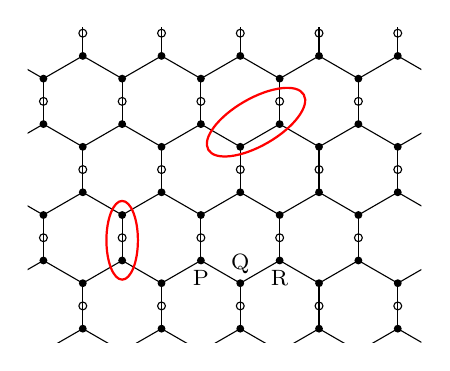
\begin{tikzpicture}

%\useasboundingbox (-1.3,-1.2) rectangle (11.2,4.7);
%	\draw (-1.5,-2.5) rectangle (3.5,7.5);

  
 \clip (-2mm,4mm) rectangle ++ (5cm, 4cm);  
   
 \foreach \u in {1,2,...,7}{%  
     \foreach \v in {1,2,...,5}{%  
          \draw ({\u + \v * cos(120)}, {\v * sin(120)} )  circle (0.5mm);
           \fill ({\u + \v * cos(120)}, {\v * sin(120) + 0.5 *  tan(30)} )  circle (0.5mm) node (o\u\v) {};
           \fill ({\u + \v * cos(120)}, {\v * sin(120) -  0.5* tan(30)} )   circle (0.5mm)node (u\u\v) {};
          \draw ({\u + \v * cos(120)}, {\v * sin(120) -  0.5* tan(30)} ) --   ++ (90:{tan(30)});
          \draw ({\u + \v * cos(120)}, {\v * sin(120) -  0.5* tan(30)} ) --   ++ (-30:{tan(30)});
          \draw ({\u + \v * cos(120)}, {\v * sin(120) -  0.5* tan(30)} ) --   ++ (-150:{tan(30)}); 
     }
  }
  
  \draw[thick, red,rotate around={30:(2.7,3.2) } ] (2.7,3.2) ellipse (7mm and 3mm);
  \draw[thick, red] (1,1.7) ellipse (2mm and 5mm);

  \node[below] at (u32) {\footnotesize P};  
  \node[below] at (u42) {\footnotesize R};  
  \node[above] at (o31) {\footnotesize Q};  
  
  

  \end{tikzpicture}




